\documentclass{article}
\usepackage{amsmath}
\usepackage{amssymb}
\usepackage{fullpage}
\usepackage{graphicx}
\usepackage{html}

\newcommand{\pivc}{$\pi$VC\ }

\begin{document}

\title{\Large CS 156 \pivc Tutorial}
\date{}
\author{\small\begin{tabular}[t]{c@{\extracolsep{8em}}c}
Jason Auerbach & Joel Galenson\\
jasonaue@stanford.edu & joel486@stanford.edu\\
OHs: & OHs:\\
Sometime & Some other time % TODO: Add
\end{tabular}}
\maketitle

\subsection*{Running and Using \pivc}

You can run \pivc on any of the \texttt{myth} or \texttt{vine} machines.  To run it, simply type \texttt{/usr/class/cs156/piVC}.  Since it launches a graphical frontent, you will need to either be at the machine itself, have X forwarded, or be running VNC.  If you need help setting this up, email one of us.
% TODO: Does it work on any of the other systems?  Not for Joel.

\pivc is easy to use (although hard to master!).  Simply open or start typing a Pi program in the left pane.  When you compile it, if there are no compile errors, \pivc will generate all the verification conditions in your code and see how many are valid.  This information will be given to you in the \texttt{Verification Conditions} tab in the right pane.  You can use the drop-down box to see which VCs are invalid and the information in the text pane below it to figure out how to make it valid.

The website for \pivc is 
\htmladdnormallink{http://theory.stanford.edu/$\sim$arbrad/pivc/index.html.}{http://theory.stanford.edu/~arbrad/pivc/index.html}
You can visit the site for another tutorial and some more programs to solve.

\subsection{An example of using \pivc}

We will present an example of using \pivc to verify the \texttt{Abs} program.  First start \pivc as shown above and then open the \texttt{/usr/class/cs156/abs.pi} file.

\begin{center}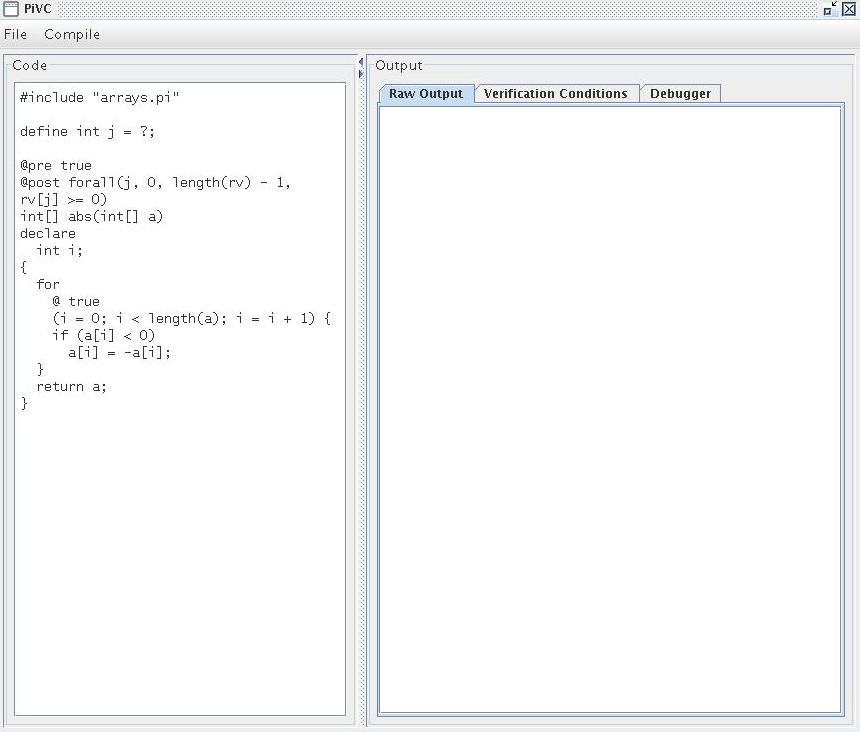
\includegraphics[width=100mm]{pivc1}\end{center}

We see that the function specification is provided for us.  There is no precondition, since \texttt{abs} can take in any array, and the postcondition specifies that each element in the returned array is non-negative.  Let's first try compiling it and seeing what happens.  It looks like not all the verification conditions are valid.  Switching to the tab on the right, we can use the drop-down box to see that there are four VCs in this function, and one of them is invalid.  Selecting it highlights it on the left and displays the corresponding basic block and the actual VC in the right.

\begin{center}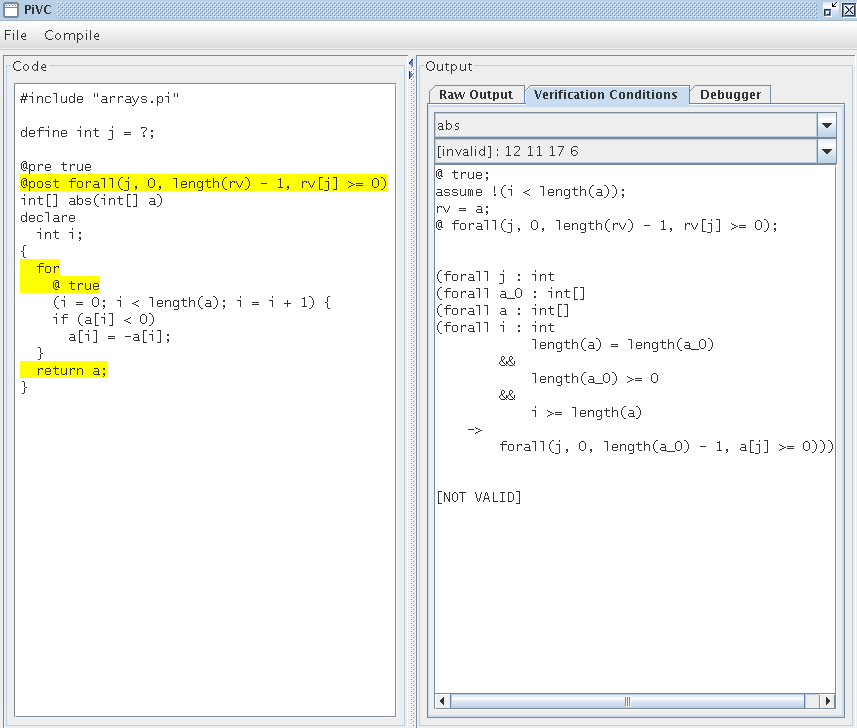
\includegraphics[width=100mm]{pivc2}\end{center}

Looking at the failing VC, we can see that it starts at the \texttt{for} loop, breaks out of it, and returns from the function.  Since the loop assertion is \texttt{true}, of course the function postcondition won't hold.  We need to give \pivc some information about what the loop is doing.  As programmers, we know that loop is walking down the array and ensuring each element in turn is non-negative, so we can supply that in an annotation and try recompiling.

\begin{center}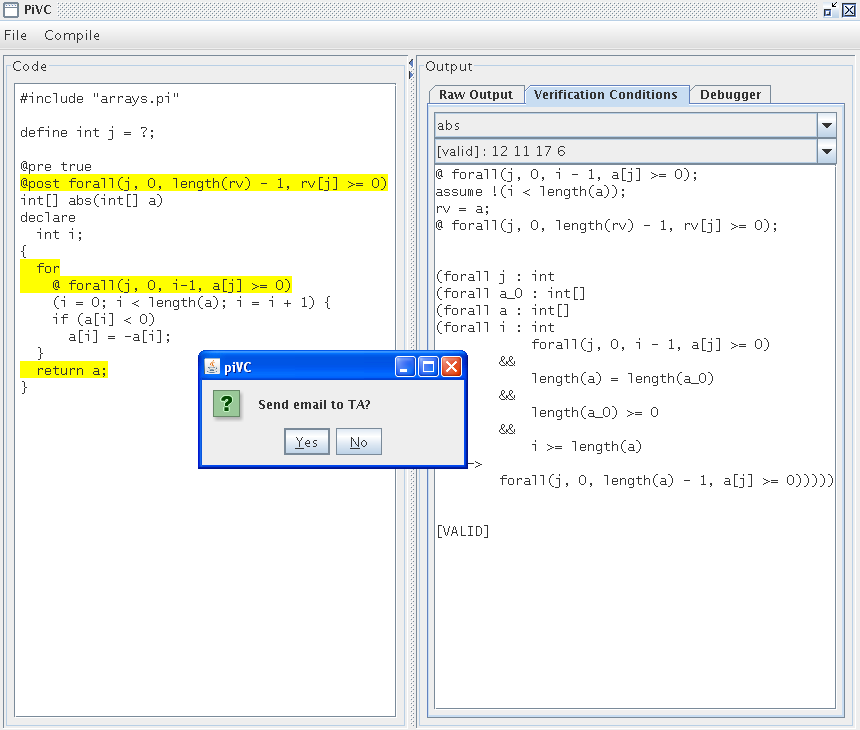
\includegraphics[width=100mm]{pivc3}\end{center}

We did it!  If this is a homework assignment, you can tell \pivc to email your solution to the TAs.

\subsection*{Tips on using \pivc}

We've just walked through proving our first program using \pivc.  That wasn't so hard, was it?  Unfortunately, \texttt{abs} is a very simple program, and most other programs are harder to prove correct.  Here are a few tips and strategies to help you out.

\begin{itemize}
\item One good strategy is to first start by supplying bounds on all the loop variables (e.g. \texttt{i}, \texttt{j}, and so forth.  You usually need these, and you'll be sure not to forget them if you start with them.
\item Remember that a basic path is generated for when we break out of a loop.  So if you have a loop
\texttt{(i = 0; i < u; i = i + 1)},
a basic path will be generated for when \texttt{i == u}.  Keep this in mind when writing an annotation for \texttt{i}'s bound.
\item The text pane in the right that shows the basic path and the VC is an invaluable tool for figuring out why a VC is not valid.  Walk through the path and the VC in your head and try to figure out why the logic doesn't hold and what you'd have to add to make it valid.
\item Another strategy is to start by going through the program and annotating everything with what you as a programmer know it does.  This way, you should have all the main loop assertions and can focus on providing the extra information needed to prove everything valid.
\item The \texttt{sorted} predicate is defined on page 120 of the book and the \texttt{partitioned} predicate is defined on page 127. % TODO: Check page numbers
\item Keep at it.  Some programs and properties can be very hard to prove, but if you keep working at it you'll eventually manage it.  Good luck!
\end{itemize}

\end{document}